\vspace{-1mm}
\section{Experiments}
\label{sec:expt}

\vspace{-1mm}
\subsection{Experimental Setup}
\label{sec:experiment_details}
\textbf{Model Architectures.}
We train two 
% transformer 
models from scratch, i.e., $\text{FILIP}_{\text{base}}$ and $\text{FILIP}_{\text{large}}$. 
The model architectures follow
% is designed to be the same as 
CLIP \citep{radford2021learning}, i.e., the image encoder is ViT-B/32 for $\text{FILIP}_{\text{base}}$ and ViT-L/14 for $\text{FILIP}_{\text{large}}$. More details can be found in Appendix \ref{apdx:expt_setting}.
% \hou{For $\text{FILIP}_{base}$, the image encoder is ViT-B/32 and the text encoder is a GPT-like model with 12 layers, embedding size 512 and 8 attention heads in each Transformer block.
% For $\text{FILIP}_{large}$, the image encoder is ViT-L/14 and the text encoder is a GPT-like model with 12 layers, embedding size 768 and 12 attention heads.
% }
% The image encoder of $\text{FILIP}_{base}$ and $\text{FILIP}_{large}$ are ViT-B/32 and ViT-L/14 separately.

\textbf{Pre-training Details.}
To save memory and scale up the batch size, automatic mixed-precision \citep{micikevicius2018mixed} and gradient checkpoint \citep{griewank2000algorithm, chen2016training} are used
The input images are resized to $224 \times 224$ resolution during pre-training and the maximum length of the text is limited to $77$ tokens following \citet{radford2021learning}.
The training is mainly conducted on Nvidia V100 GPUs and Ascend Cards.
$\text{FILIP}_{\text{base}}$ is trained on 128 cards about 9 days and $\text{FILIP}_{\text{large}}$ takes about 24 days to train on 192 cards. 
Unless otherwise specified, we use $\text{FILIP}_{\text{large}}$ to compare with other methods and $\text{FILIP}_{\text{base}}$ for ablation.
We train both models using the LAMB optimizer \citep{2019Large} and cosine learning rate schedule \citep{2016SGDR} with a linear warmup. 
Weight decay regularization is applied to all parameters except bias, layer normalization, token embedding, positional embedding and temperature in contrastive loss. 
% More details of 
Detailed values of hyperparameters for different datasets and models can be found in Appendix \ref{apdx:expt_setting}.


%Similar to \cite{radford2021learning}, we also add one extra epoch to pretrain $\text{FILIP}_{base}$ on the images with 336 x 336 resolution. We denote this model as $\text{FILIP}_{large+}$ 
% $$
% lr = lr_{base} * \sqrt{2}^{\log{batchsize/ 512}}
% $$

\vspace{-1mm}
\subsection{Zero-Shot Image Classification}
\label{sec:zeroshot_classification}
In this section, we evaluate our proposed FILIP on the zero-shot image classification task.
We compare our FILIP with CLIP \citep{radford2021learning} on 12 downstream classification datasets, using the same evaluation setting as in CLIP. As described in Section \ref{sec:prompt_ensemble}, we  apply a set of prompts for each dataset and ensemble them to get the final results, see Appendix \ref{apdx:prompt_template} for details. We only compare the zero-shot performance with CLIP here as ALIGN does not release its model and  the related performances are not reported in their paper.

Table \ref{zeroshot-classification-table} shows the results on 12 datasets.
Despite using less training data (340M vs. 400M), both $\text{FILIP}_{\text{base}}$ and $\text{FILIP}_{\text{large}}$ considerably outperform their CLIP counterparts in terms of average top-1 accuracy over 12 datasets, i.e., achieving  absolute improvements of 5.6\% and 3.0\%, respectively. In particular, our FILIP surpasses CLIP on  ImageNet, the largest dataset among 12 datasets.
% by a large margin 
FILIP also achieves substantial performance gains on some domain-specific datasets, e.g., for Aircrafts, the two FILIP models reach a 30\% improvement over CLIP on average. We speculate this is because,
unlike CLIP which aggregates the information of the whole image into the representation of the [CLS] token, our proposed FILIP model focuses more on the target object by directly aligning the image patches corresponding to the target object with the textual tokens corresponding to the class label (visualizations of word-patch alignment are in Section \ref{sec:Visualization of Fine-grained Alignment}).

% Although classification task  mainly relies on global representation of the main object, 
% we still emphasize FILIP's capability of capturing fine-grained information, which will be discussed 
% in later Section \ref{sec:Visualization of Fine-grained Alignment}. 

% We speculate the improvements can be attributed to the FILIP's capability of capturing finer-grained information, which will be further discussed in the later Section \ref{sec:Visualization of Fine-grained Alignment}.\footnote{\hou{does the visualization has discussion on this dataset? better add some to support this speculation}}

\begin{table}
\vspace{-3mm}
\center
\caption{Results of zero-shot image-text retrieval on Flickr30K and MSCOCO datasets. The last two rows (marked with *) report the zero-shot results on Flickr30K dataset of model fine-tuned on MSCOCO dataset, following the setting of ALBEF \citep{li2021align}.}
\huge
\label{tab:zero-shot-retrieval-table}
\resizebox{\textwidth}{!}{
\begin{tabular}{ccccccccccccc}
\toprule
            & \multicolumn{6}{c}{Flickr30K}                                                               & \multicolumn{6}{c}{MSCOCO}                                                                  \\
            & \multicolumn{3}{c}{image-to-text} & \multicolumn{3}{c}{text-to-image} & \multicolumn{3}{c}{image-to-text} & \multicolumn{3}{c}{text-to-image} \\
            & R@1           & R@5           & R@10         & R@1           & R@5           & R@10         & R@1           & R@5           & R@10         & R@1           & R@5           & R@10         \\
\midrule
Unicoder-VL & 64.3          & 85.8          & 92.3         & 48.4          & 76.0            & 85.2         & $-$             & $-$             & $-$            & $-$             & $-$             & $-$            \\
ImageBERT   & 70.7          & 90.2          & 94.0           & 54.3          & 79.6          & 87.5         & 44.0            & 71.2          & 80.4         & 32.3          & 59.0            & 70.2         \\
UNITER      & 83.6          & 95.7          & 97.7         & 68.7          & 89.2          & 93.9         & $-$             & $-$             & $-$            & $-$             & $-$             & $-$            \\
CLIP        & 88.0            & 98.7          & 99.4         & 68.7          & 90.6          & 95.2         & 58.4          & 81.5          & 88.1         & 37.8          & 62.4          & 72.2         \\
ALIGN       & 88.6          & 98.7          & 99.7         & \textbf{75.7}          & \textbf{93.8}          & \textbf{96.8}         & 58.6          & 83.0            & 89.7         & 45.6          & 69.8          & 78.6         \\
\textbf{FILIP}      & \textbf{89.8}          & \textbf{99.2}          & \textbf{99.8}         & {75.0}            & {93.4}          & {96.3}         & \textbf{61.3}          & \textbf{84.3}          & \textbf{90.4}         & \textbf{45.9}          & \textbf{70.6}          & \textbf{79.3}         \\ \hline
ALBEF*       & 94.1          & 99.5          & 99.7         & 82.8          & 96.3          & 98.1         & $-$             & $-$             & $-$            & $-$             & $-$             & $-$            \\
\textbf{FILIP}*       & \textbf{95.4}          & \textbf{99.8}          & \textbf{100.0}         & \textbf{84.7}            & \textbf{97.0}          & \textbf{98.7}         & $-$             & $-$             & $-$            & $-$             & $-$             & $-$            \\
\bottomrule         
\end{tabular}}
\vspace{-3mm}
\end{table}



\vspace{-1mm}
\subsection{Image-Text Retrieval}
\label{sec:image_text_retrieval}
Image-text retrieval consists of two sub-tasks: image-to-text retrieval and text-to-image retrieval. 
We evaluate our FILIP model on two retrieval benchmark datasets: Flickr30K \citep{dataset_flickr30k} and MSCOCO \citep{dataset_mscoco}, under both zero-shot and fine-tuned settings. 
% We follow the Karpathy split \citep{karpathy2015deep} for both datasets. 
More details of experimental setting can be found in Appendix \ref{apdx:expt_setting}.

Tables \ref{tab:zero-shot-retrieval-table} and  \ref{tab:finetuned-retrieval-table} show the results of 
zero-shot and fine-tuned 
image-text retrieval,
respectively. We compare our FILIP model against methods with complex attention layers including Unicoder-VL \citep{unicoder_vl}, ImageBERT \citep{imagebert}, UNITER \citep{chen2020uniter}, VILLA \citep{villa}, ERNIE-ViL \citep{ernie_vil}, Oscar \citep{li2020oscar}, VinVL \citep{zhang2021vinvl}, ALBEF \citep{li2021align}, and methods trained on larger-scale image-text datasets including CLIP \citep{radford2021learning} and ALIGN \citep{jia2021scaling}. As we can see, FILIP achieves state-of-the-art performances under all metrics on both Flickr30K and MSCOCO datasets, except for zero-shot text-to-image retrieval on Flickr30K, where FILIP achieves competitive performance with SOTA. For zero-shot image-to-text retrieval on MSCOCO dataset, the absolute R@1 of our proposed FILIP is 2.7\% higher than ALIGN, which is trained on a much larger dataset.

\begin{table}
\vspace{-3mm}
\center
\caption{Results of 
fine-tuned 
image-text retrieval on Flickr30K and MSCOCO datasets.}
% \hou{with finetuning}.}
\Large
\label{tab:finetuned-retrieval-table}
\resizebox{\textwidth}{!}{
\begin{tabular}{ccccccccccccc}
\toprule
            & \multicolumn{6}{c}{Flickr30K}                                                               & \multicolumn{6}{c}{MSCOCO}                                                                  \\
            & \multicolumn{3}{c}{image-to-text} & \multicolumn{3}{c}{text-to-image} & \multicolumn{3}{c}{image-to-text} & \multicolumn{3}{c}{text-to-image} \\
            & R@1           & R@5           & R@10         & R@1           & R@5           & R@10         & R@1           & R@5           & R@10         & R@1           & R@5           & R@10         \\
\midrule
Unicoder-VL & 86.2          & 96.3          & 99.0           & 71.5          & 90.9          & 94.9         & 62.3          & 87.1          & 92.8         & 48.4          & 76.7          & 85.9         \\
ImageBERT   & 87.0            & 97.6          & 99.2         & 73.1          & 92.6          & 96.0           & 66.4          & 89.8          & 94.4         & 50.5          & 78.7          & 87.1         \\
UNITER      & 87.3          & 98.0            & 99.2         & 75.6          & 94.1          & 96.8         & 65.7          & 88.6          & 93.8         & 52.9          & 79.9          & 88.0           \\
VILLA       & 87.9          & 97.5          & 98.8         & 76.3          & 94.2          & 96.8         & $-$             & $-$             & $-$            & $-$             & $-$             & $-$            \\
ERNIE-ViL   & 88.1          & 98.0            & 99.2         & 76.7          & 93.6          & 96.4         & $-$             & $-$             & $-$            & $-$             & $-$             & $-$            \\
% GPO         & 88.7          & 98.9          & 99.8         & 76.1          & 94.5          & 97.1         & 68.1          & 90.2          & $-$            & 52.7          & 80.2          & $-$            \\
Oscar       & $-$             & $-$             & $-$            & $-$             & $-$             & $-$            & 73.5          & 92.2          & 96.0           & 57.5          & 82.8          & 89.8         \\
VinVL       & $-$             & $-$             & $-$            & $-$             & $-$             & $-$            & 75.4          & 92.9          & 96.2         & 58.8          & 83.5          & 90.3         \\
ALIGN       & 95.3          & 99.8          & 100.0          & 84.9          & 97.4          & 98.6         & 77.0            & 93.5          & 96.9         & 59.9          & 83.3          & 89.8         \\
ALBEF       & 95.9          & 99.8          & \textbf{100.0}          & 85.6          & 97.5          & 98.9         & 77.6          & 94.3          & 97.2         & 60.7          & \textbf{84.3}          & 90.5         \\
Our FILIP       & \textbf{96.6}          & \textbf{100.0}          & \textbf{100.0}          & \textbf{87.1}          & \textbf{97.7}          & \textbf{99.1}         & \textbf{78.9}          & \textbf{94.4}          & \textbf{97.4}         & \textbf{61.2}          & \textbf{84.3}          & \textbf{90.6}        \\
\bottomrule
\end{tabular}}
\vspace{-3mm}
\end{table}



\begin{table}
\vspace{-3mm}
\caption{Ablation study of different components on pre-training subset of YFCC100M. I2T and T2I are abbreviations for image-to-text and text-to-image retrieval, respectively. ``ZS'' means zero-shot performance. Underlined numbers have
the highest improvements for the corresponding metrics. }
\label{ablation-yfcc-table}
\begin{center}
\begin{tabular}{l|rrrrr}
\toprule \multirow{2}{*}{ Model } & \multicolumn{4}{c} { MSCOCO }         & ImageNet \\
                                 & I2T R@1 & I2T R@5 & T2I R@1 & T2I R@5 & ZS Top1 \\
\midrule Baseline (ViT-B/32) & $25.0$ & $49.5$ & $14.7$ & $34.7$ & 30.4 \\ % $32.5$ 
~w/ image augmentation & $26.1$ & $51.8$ & $16.5$ & $37.5$ & $ 32.5 $ \\  % \underline{36.7}
~w/ back translation & $29.2$ & $55.0$ & $17.9$ & $39.8$ & $33.9$ \\ % $37.0$ 
% ~w/ interaction layers & $26.6$ & $52.2$ & $16.3$ & $36.8$ & $34.0$ \\
~w/ cross-modal late interaction & $\underline{30.5}$ & $\underline{55.3}$ & $\underline{18.5}$ & $\underline{40.0}$ & $\underline{34.3}$\\
Our $\text{FILIP}_{\text{base}}$ & $\mathbf{33.4}$ & $\mathbf{60.1}$ & $\mathbf{23.0}$ & $\mathbf{46.2}$ & $\mathbf{37.8}$ \\  % $\mathbf{40.3}$
\bottomrule
\end{tabular}
\end{center}
\vspace{-3mm}
\end{table}


\begin{table}[t!]
\vspace{-3mm}
    \caption{Efficiency study of the cross-modal late interaction. ``orig'' and ``late'' stand for the contrastive loss based on the original cosine similarity 
    in CLIP and our proposed cross-modal late interaction, respectively. ``ZS'' means zero-shot performance.
    We report results for ViT-B/32 trained on filtered YFCC100M with 8 V100 GPUs, with a batch size of 512 per GPU. Training time and memory consumption are tested using the same gradient checkpoint configuration. 
    % The setting with 
    * denotes our final setting used in other experiments.}
    \label{tab:efficiency-late}
    \begin{center}

    \begin{tabular}{cccccccc}
    \toprule \multirow{2}{*}{ Loss }   &Embed&Embed &  Token  &  Training time   &  Memory  & ImageNet \\
                                     & dim & precision&  \% & (sec/iter)     &  (MB)    & ZS Top1  \\
    \midrule 
    orig (baseline)& 512 & fp32 & - &1.31 & 14300  & 30.4 \\
    late & 512 & fp32 &100\% & 2.85 & 26000 & 34.6 \\
    late & 512 & fp16 &100\% & 2.67 & 23468 & 34.5 \\
    late & 256 & fp16 &100\% & 2.31 & 22382 & \textbf{35.2} \\
    late & 256 & fp16 &50\% & 1.61 & 16336 & 34.5 \\
    late* & 256 & fp16 &25\% & 1.39 & 16100 & 34.3 \\
    % \midrule 
    % orig (baseline)&  $512\times128 $ & 512 & - &   & & - \\
    % late&  $512\times128 $  & 256 & 25\% & &  & - \\
    
    \bottomrule
    \end{tabular}
    \end{center}
    \vspace{-3mm}
\end{table}

\vspace{-1mm}
\subsection{Ablation Study}
\label{sec:ablation_yfcc}

\textbf{Effectiveness of Each Component.}
% In this section,
We study the effectiveness of each component  in FILIP, i.e., image/text augmentations and cross-modal late interaction. Experiments are conducted on 
% ViT-B/32 
$\text{FILIP}_{\text{base}}$,
with a filtered subset of YFCC100M as the training dataset (as described in Section \ref{sec:dataset_construction}),
on both zero-shot retrieval and classification tasks. 
% Unless otherwise specified, this setting\footnote{\hou{which setting?}} is also used for experiments in the later sections. 
We measure models' performance on  MSCOCO zero-shot image-text retrieval and ImageNet zero-shot classification, which are two effective indicators 
for the quality of the learned vision-language representations. 

Table \ref{ablation-yfcc-table} reports the results. As can be seen, all three components 
are beneficial for both tasks.
Despite the simple design, cross-modal late interaction brings significant performance improvements over the baseline (the vanilla CLIP ViT-B/32), with an absolute R@1 gain of 5.5\% (resp. 3.8\%)  for image-to-text (resp. text-to-image) retrieval on MSCOCO and an absolute top-1 accuracy gain of 3.9\% for zero-shot classification on ImageNet. 
Further improvements are observed when all components are combined together.
% When all components are combined together, substantial improvements can be observed for both tasks.

% \footnote{\hou{remove this discussion currently because retrival requires finer-grained matching is not well-supported, discussing too much might over-claim.}}

% For zero-shot classification,  the augmentation techniques are more effective, bringing 4.2\% \hou{absolute} gains in top-1 accuracy; while retrieval task, for which a finer-grained matching is required, 
% \hou{benefits more from the cross-modal late interaction,}
% getting 4.8\% and 8.3\% \hou{absolute} R@1 improvements for image-to-text and text-to-image retrieval, respectively. 
% This indicates that our late interaction loss is effective to capture the fine-grained token-wise correspondence between texts and images, while is also efficient compared to other fully-interaction models.



\begin{figure}
\vspace{-3mm}
	\centering
	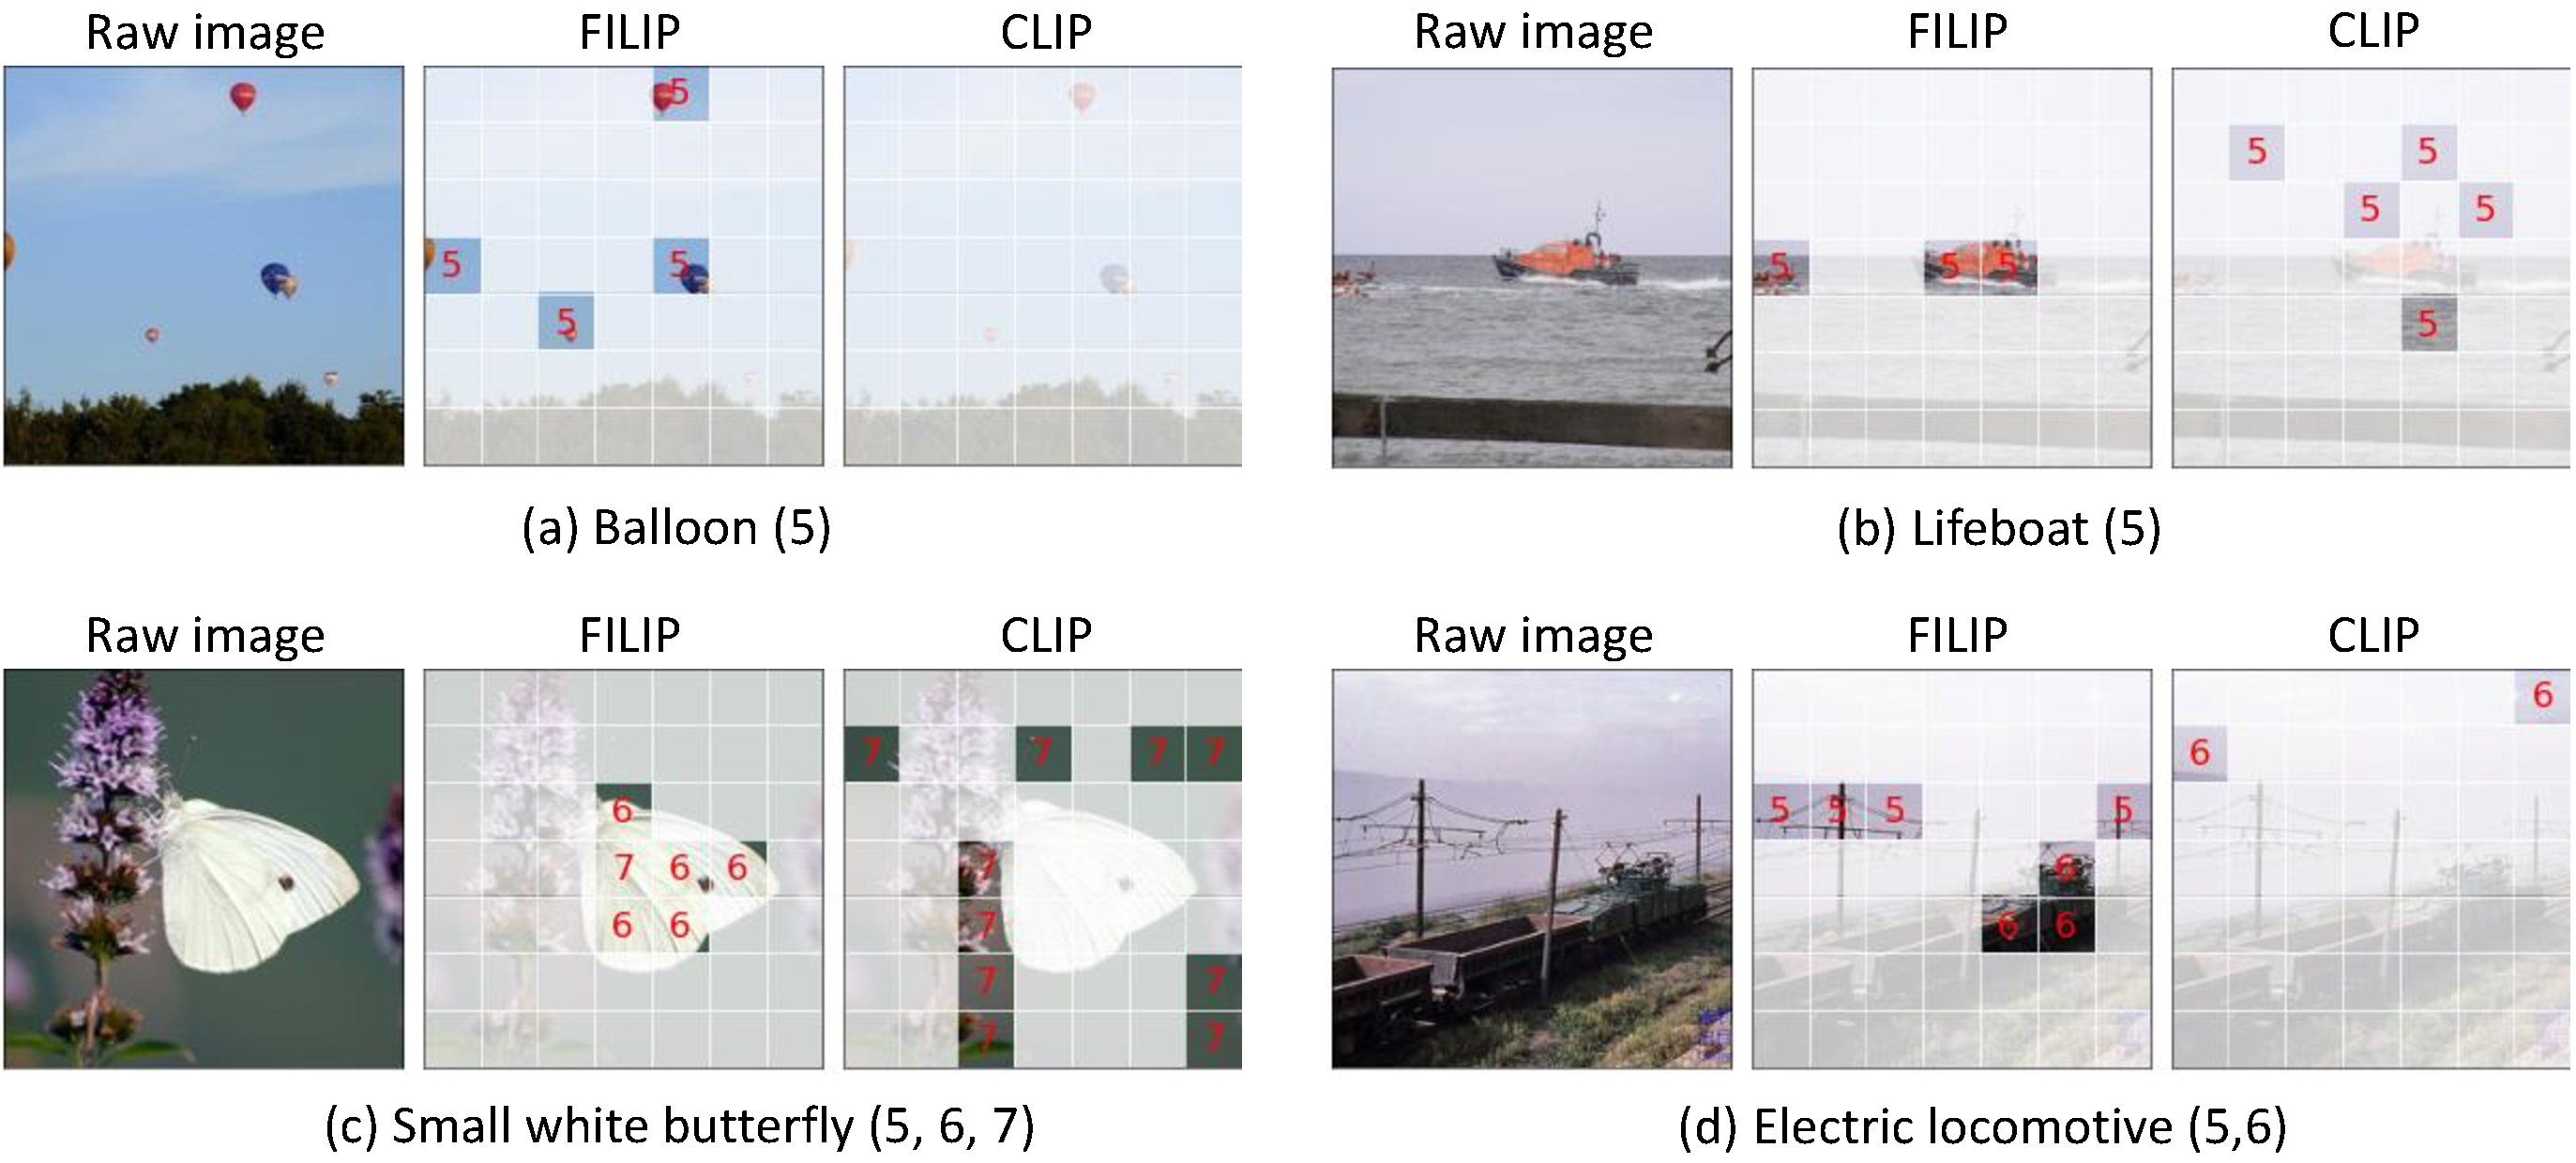
\includegraphics[width=\linewidth]{figures/ImageNetVis_vsCLIP.pdf}
	\vspace{-5mm}
	\caption{Visualizations of word-patch alignment for 4 classes of the ImageNet dataset and ``a photo of a \{label\}." is the prompt. Numbers in the parentheses after the class label indicate the location indices of the class label in the tokenized textual sequence. The correct predictions are highlighted by opaque patches with the class label indices in red.}
	\label{fig:single_obj}
	\vspace{-3mm}
\end{figure}


\textbf{Efficiency Study of Cross-modal Late Interaction.}
\label{sec:efficiency-study-of-late-loss}
% Efficiency is a crucial issue for the 
% late interaction mechanism in Section~\ref{sec:Cross-modal-late}, as
Since the late interaction mechanism in Section~\ref{sec:Cross-modal-late} requires to calculate the similarity between all visual and textual tokens, 
its efficiency can be a problem when
employed in large-scale distributed training.
% late interaction loss without efficiency optimization can bring considerable computational overhead compared to the original contrastive loss. 
As described in Section \ref{sec:Cross-modal-late}, we make several attempts to address the issue. 
Table \ref{tab:efficiency-late} shows the efficiency improvement on zero-shot classification on ImageNet when
% in terms of training time and memory consumption when
% studies the trade-off between efficiency and accuracy of 
these attempts are applied. 
As can be seen, these attempts improve the efficiency of late interaction  
without accuracy drop. Combining all three attempts achieves only slightly slower training and larger memory consumption than the original loss in CLIP.

% \ylw{[finish the table when the server is available and write some conclusions here]} \hou{add observations when results are ready.}

\vspace{-1mm}
\subsection{Visualization of Fine-grained Alignment}
\label{sec:Visualization of Fine-grained Alignment}

In this section, we visualize FILIP's capability of capturing fine-grained cross-modal correspondence using the method of word-patch alignment. To make a fair comparison, we use our $\text{FILIP}_{\text{base}}$ trained on YFCC100M and CLIP's ViT-B/32, which are of the same size, for visualization. Each image is patchified to $7\times 7$ image patches. 
More visualization results can be found in Appendix~\ref{apdx:more_vis}.

\textbf{Visualization Method.} The word-patch alignment is performed based on the token-wise similarity between the image patches and textual tokens. Specifically, for the $k$-th image patch, the location index of textual token   with the largest similarity with it ($m_k^I$ in Equation~(\ref{eq:late_sim_i})) is considered as its predicted label, and is placed at the center of it.
% each image patch.
Take class ``balloon'' as an example. 
There are 8 tokens in the tokenized textual sequence ``[BOS] a photo of a balloon. [EOS]'', 
and the location index of the class label ``balloon'' is ``5''. 
Note that one class label may be tokenized to more than one token.
% For word-patch alignment, 
% the predicted label is placed at the center of each image patch.
Location indices of textual tokens corresponding to the class label are highlighted in red, while the others are marked in white.
A desired model that learns fine-grained representations  would predict  image patches of the target object to red indices.

\textbf{Observations.}
Figure~\ref{fig:single_obj} shows the word-patch alignment results for FILIP and CLIP on 4 classes from the ImageNet dataset.
% For word-patch alignment, the predicted label is placed at the center of each image patch.
% \houTextual token indexes corresponding to the class label are highlighted in red, while the others are marked in white.
As can be seen,
% from Figure~\ref{fig:MoreImageNetVis}, 
FILIP exhibits the finer-grained understanding of 
an image in the following aspects. 
(i) A single object: 
% As 
% can be seen 
From the visualization of class ``small white butterfly'', the image patches covering the object are all classified correctly;
% to textual token indexes corresponding to the class label. 
(ii) Same object in different shapes:
From the visualizations of class ``balloon'' and ``lifeboat'', image patches corresponding to all target objects with different shapes and locations  are correctly classified; 
(iii) Key Components of an object: For class ``electric locomotive'', there are two key components crucial to correctly classifying the image, i.e., ``electric'' and ``locomotive'', whose corresponding textual token indices are ``5'' and ``6'', respectively. As can be seen, image patches matching these two key components are respectively correctly classified.
On the other hand, CLIP can not correctly align image patches with corresponding textual tokens.
%Similar as \cite{kim2021vilt}. 
Compared with \cite{kim2021vilt} which uses an extra optimal transport to align the textual word and image patch distributions, the word-patch alignment can be simply automatically learned by our method. 


% In this section, we visualize the cross-modal alignment of the proposed method, in terms of
% both  word-patch alignment and Grad-CAM heatmaps~\citep{selvaraju2017grad}.
% \paragraph{Visualization Method.} The word-patch alignment is performed based on the token-wise similarity between the image patches and textual tokens. Specifically, for the $k$-th image patch, the textual token index  with the largest similarity with it ($m_k^I$ in Equation~(\ref{eq:late_sim_i})) is considered as its 
% % patch-level
% predicted label.
% % \paragraph{Grad-cam Visualization.} 
% We compute the Grad-CAM heatmaps based on the average self-attention maps over the image patches classified to targeted textual tokens (i.e., the textual token(s) corresponding to the class label in the ImageNet dataset) in the last layer of the image encoder. We average the heatmaps over all attention heads.

% \paragraph{Observations.}
% Figure~\ref{fig:single_obj} shows the word-patch alignment and Grad-CAM visualization (More examples on more classes can be found in Appendix~\ref{apdx:more_vis}), using the model trained on YFCC100M dataset
% % top50_top50_256 / top25_top25_pickinall_3
% on class "damselfly" of the ImageNet dataset. 
% %  More visualizations on more images from more classes can be found in Appendix~\ref{apdx:more_vis}.
% For word-patch alignment, the predicted label  is placed at the center of each image patch.
% Textual token indexes corresponding to the class label are highlighted in red, while the others are marked in white.
% Note that one class label may be tokenized to more than one token.

% As can be seen from Figure~\ref{fig:MoreImageNetVis}, our proposed model exhibits the finer-grained understanding of 
% an image in several aspects. 
% (i) A single object: As can be seen from the visualization of class ``small white butterfly, the image patches covering the object are all classified correctly to textual token indexes corresponding to the class label. 
% (ii) Same object in different shapes: Three image patches corresponding to balloons with different shapes and locations  are correctly classified;
% (iii) Key Components of an object: For class ``electric locomotive'', there are two key components to correctly classify the image, i.e., ``electric'' and ``locomotive'' whose corresponding textual token indices are ``5'' and ``6'', respectively. As can be seen, image patches matching these two key components are respectively correctly classified.
% %Similar as \cite{kim2021vilt}. 
% Compared with \cite{kim2021vilt} which uses an extra optimal transport to align the textual word and image patch distributions,  the word-patch alignment can be simply automatically learned by using the proposed late interaction mechanism. 

% \subsection{Image Captioning}
% \label{sec:image_caption}
% \begin{table}
% \center
% \caption{Results of fine-tuned image captioning on MSCOCO karpathy test split \citep{2016Deep}.}
% % \hou{with finetuning}.}
% \label{tab:caption_result}
% \begin{tabular}{l|cccc}
% \toprule
% &  BlEU @ 4 & METEOR & CIDEr & SPICE \\
% \midrule % \hline 
% BUTD \citep{anderson2018bottom} & $36.3$ & $27.7$ & $120.1$ & $21.4$ \\
% VLP \citep{zhou2020unified} & $39.5$ & $29.3$ & $129.8$ & $22.4$ \\
% AoANet \citep{huang2019attention} & $38.9$ & $29.2$ & $129.8$ & $22.4$ \\
% OSCAR \citep{li2020oscar} & $41.7$ & $30.6$ & $140.0$ & $24.5$ \\
% VinVL \citep{zhang2021vinvl} & $41.0$ & $31.1$ & $140.9$ & $25.2$ \\
% \midrule % \hline 
% $\text{FILIP}_{base}$ + Bart Base & $ $ & $ $ & $ $  \\
% $\text{FILIP}_{large}$ + Bart Large & $ $ & $ $ & $ $  \\
% \bottomrule
% \end{tabular}
% \end{table}

